

We introduce hierarchically supervised latent Dirichlet allocation (HSLDA), a
model for hierarchically and multiply labeled bag-of-word data.  Examples of
such data include web pages and their placement in directories, product
descriptions and associated categories from product hierarchies, and free-text
clinical records and their assigned diagnosis codes. Out-of-sample label
prediction is the primary goal of this work, but improved lower-dimensional
representations of the bag-of-word data are also of interest.
%% We demonstrate HSLDA on large-scale data from clinical document labeling and
%% retail product categorization tasks. We show that leveraging the structure from
%% hierarchical labels improves out-of-sample label prediction substantially when
%% compared to models that do not. 

Our work operates within the framework of topic modeling. Our approach learns
topic models of the underlying data and labeling strategies in a joint model,
while leveraging the hierarchical structure of the labels. For the sake of
simplicity, we focus on is-a hierarchies, but the model can be
applied to other structured label spaces. Our work extends supervised latent Dirichlet
allocation (sLDA)~\cite{BleiMcAuliffe2008} to take advantage of hierarchical
supervision and proposes an efficient way to incorporate such information into the model. 
We hypothesize that the context of labels within
the hierarchy provides valuable information about labeling. Other models, such as LabeledLDA\citep{Ramage2009}, incorporate LDA and supervision; However, none of these models leverage dependency structure in the label space.

We demonstrate our model on large, real-world datasets in the clinical and web
retail domains. We observe that hierarchical information is valuable when
incorporated into the learning and improves our primary goal of multi-label
classification. Our results show that a joint, hierarchical model outperforms a
classification with unstructured labels as well as a disjoint model, where the
topic model and the hierarchical classification are inferred
independently of each other. 

HSLDA is a model for hierarchically, multiply-labeled, bag-of-word data.  We
will refer to individual groups of bag-of-word data as documents.  Let $w_{n,d}
\in \Sigma$ be the $n$th observation in the $d$th document.  Let $\mathbf{w}_d
= \{w_{1,d},\ldots,w_{1,N_d}\}$ be the  set of $N_d$ observations in document
$d$.  Let there be $D$ such documents and let the size of the vocabulary be
$V=|\Sigma|$.  Let the set of labels be $\mathcal{L}=\left\{
  l_{1},l_{2},\ldots,l_{\left|\mathcal{L}\right|}\right\} $. Each label labels
$l \in \mathcal{L}$, except root, has a parent $\mathrm{pa}(l) \in \mathcal{L}$
also in the set of labels. 
 We will for exposition purposes assume that this label set has hard ``is-a''
 parent-child constraints (explained later), although this assumption can be
 relaxed at the cost of more computationally complex inference.  Such a label hierarchy forms a multiply rooted tree.  Without loss of generality we will consider a tree with a single root $r\in\mathcal{L}$.  Each document has a variable $y_{l,d} \in \{-1,1\}$ for every label which indicates whether the label is applied to document $d$ or not.   In most cases $y_{i,d}$ will be unobserved, in some cases we will be able to fix its value because of  constraints on the label hierarchy, and in the relatively minor remainder its value will be observed.  In the applications we consider, only positive label applications are observed.  


%In HSLDA, the bag-of-word document data is modeled using the LDA
%mixed-membership mixture model with global topic estimation.
In HSLDA, documents are modeled using the LDA mixed-membership mixture model
with global topic estimation. Label responses are generated using a conditional
hierarchy of probit regressors\cite{gelmanbda04}. The HSLDA graphical model is given in
Figure~\ref{fig:graphical_model}. In the model, $K$ is the number of LDA
``topics'' (distributions over the elements of $\Sigma$), $\boldsymbol\phi_k$
is a distribution over ``words,'' $\boldsymbol\theta_d$ is a document-specific
distribution over topics, $\boldsymbol\beta$ is a global distribution over
topics, Dir$_{K}(\cdot)$ is a $K$-dimensional Dirichlet distribution,
$\mathcal{N}_{K}(\cdot)$ is the $K$-dimensional Normal distribution,
$\mathbf{I}_{K}$ is the $K$ dimensional identity matrix,  $\mathbf{1}_d$ is the
$d$-dimensional vector of all ones, and $\mathbb{I}(\cdot)$ is an indicator
function that takes the value $1$ if its argument is true and $0$ otherwise. 

\begin{figure}[t]
%tbp] %  figure placement: here, top, bottom, or page
 \centering 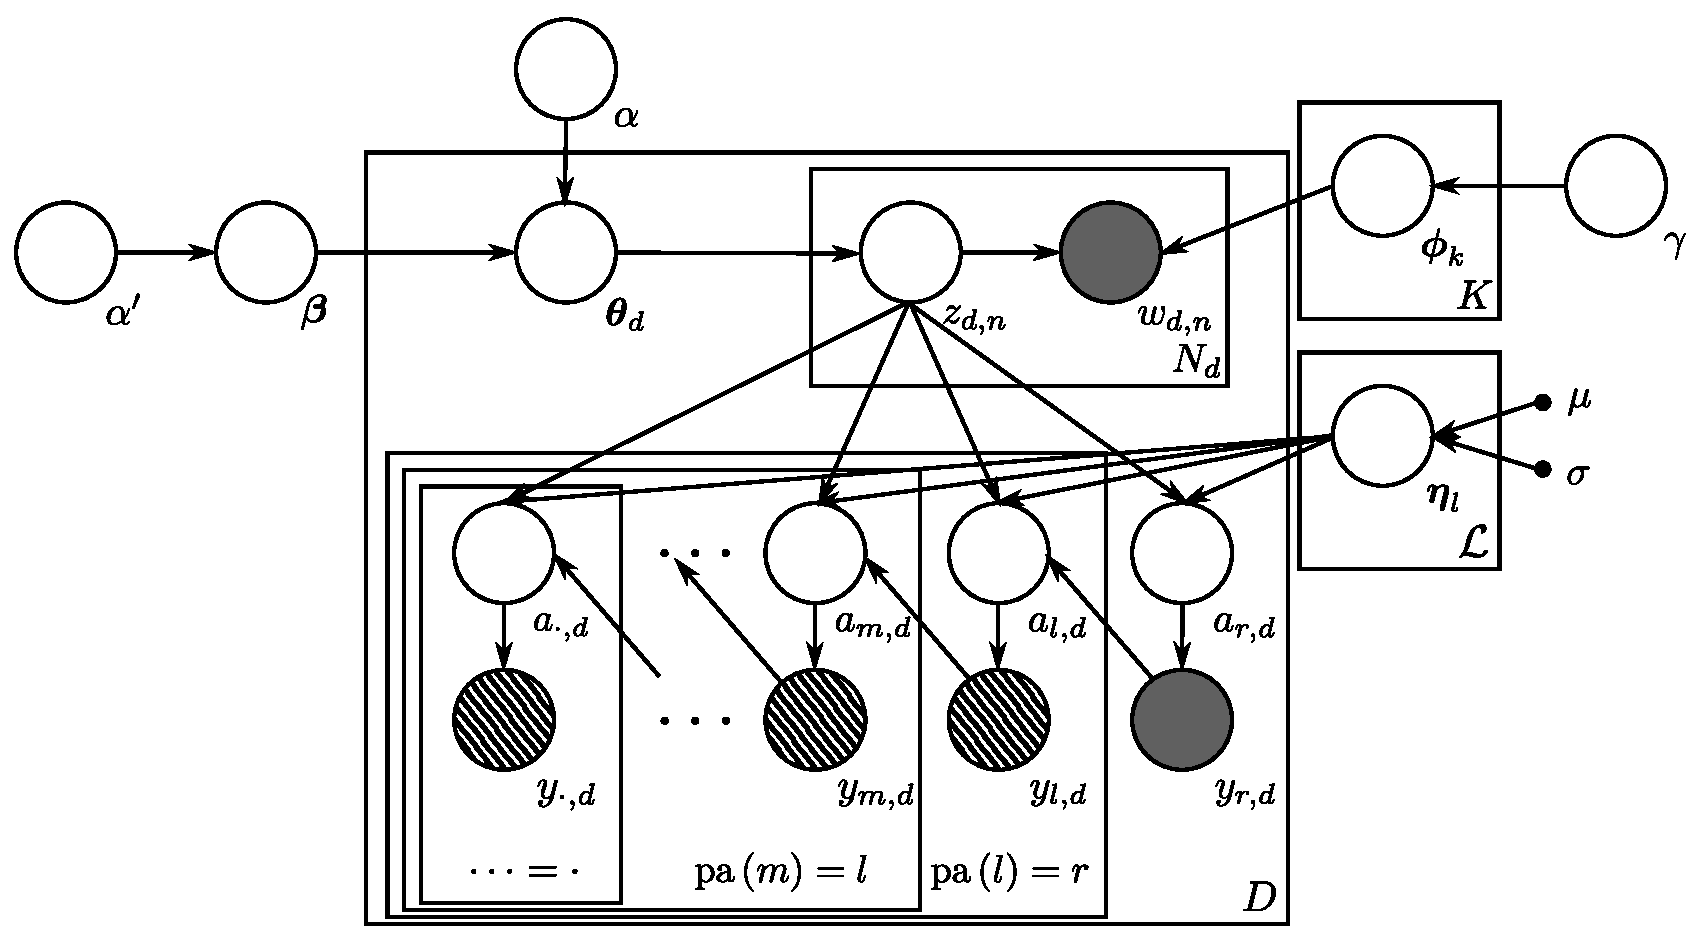
\includegraphics[scale=0.25]{Graphical_Model-final} \caption{HSLDA graphical model}


\label{fig:graphical_model} 
\end{figure}


Posterior inference in HSLDA was performed using Gibbs sampling and Markov chain Monte Carlo.  Note that, like in collapsed Gibbs samplers for LDA \cite{Griffiths04}, we have analytically marginalized out the parameters $\boldsymbol{\phi}_{1:K}$
and $\boldsymbol{\theta}_{1:D}$. HSLDA also employs a hierarchical Dirichlet prior over topic assignments (i.e.,~$\boldsymbol\beta$ is estimated from data rather than assumed to be symmetric).  This has been shown to improve the quality and stability of inferred topics \citep{WallachMiMc2009}. The hyperparameters $\alpha$, $\alpha^{\prime}$, and $\gamma$ are
%given broad ${\rm Gamma}(1,1000)$ prior distributions and 
sampled
using Metropolis-Hastings. 


We applied HSLDA to data from two domains: predicting medical
diagnosis codes from hospital discharge summaries and predicting product
categories from Amazon.com product descriptions. The clinical dataset consists
of 6,000 clinical notes along with associated billing codes that are used
to document conditions that a particular patient was treated for. These billing
codes (7298 distinct codes in our dataset) are organized in an is-a hierarchy. The retail dataset
consists of product descriptions for DVDs from the Amazon.com product catalog. This data
was partially obtained from the Stanford Network Analysis Platform (SNAP) dataset~\citep{SNAP}. The comparison models included sLDA with independent
regressors (hierarchical constraints on labels ignored) and HSLDA fit by first
performing LDA then fitting tree-conditional regressions. The number of topics for all models was set to 50, the prior distributions of
$p\left(\alpha\right)$, $p\left(\alpha^{\prime}\right)$, and
$p\left(\gamma\right)$ were gamma distributed with a shape parameter of 1 and a
scale parameters of 1000. 

\begin{figure}[h]
\begin{center}
%\subfloat[][\label{fig:1a}]{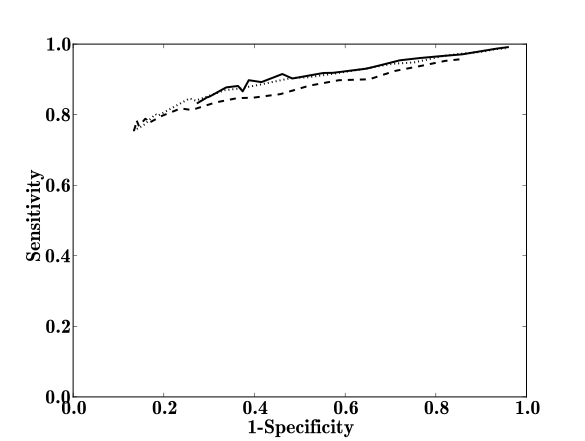
\includegraphics[width=.49\textwidth]{figs/amazon_pred_varying_mu}}
\subfigure[][]{\label{fig:1a}\includegraphics[width=.3\textwidth]{figs/clin_pred_varying_mu}}
%\subfloat[][\label{fig:1c}]{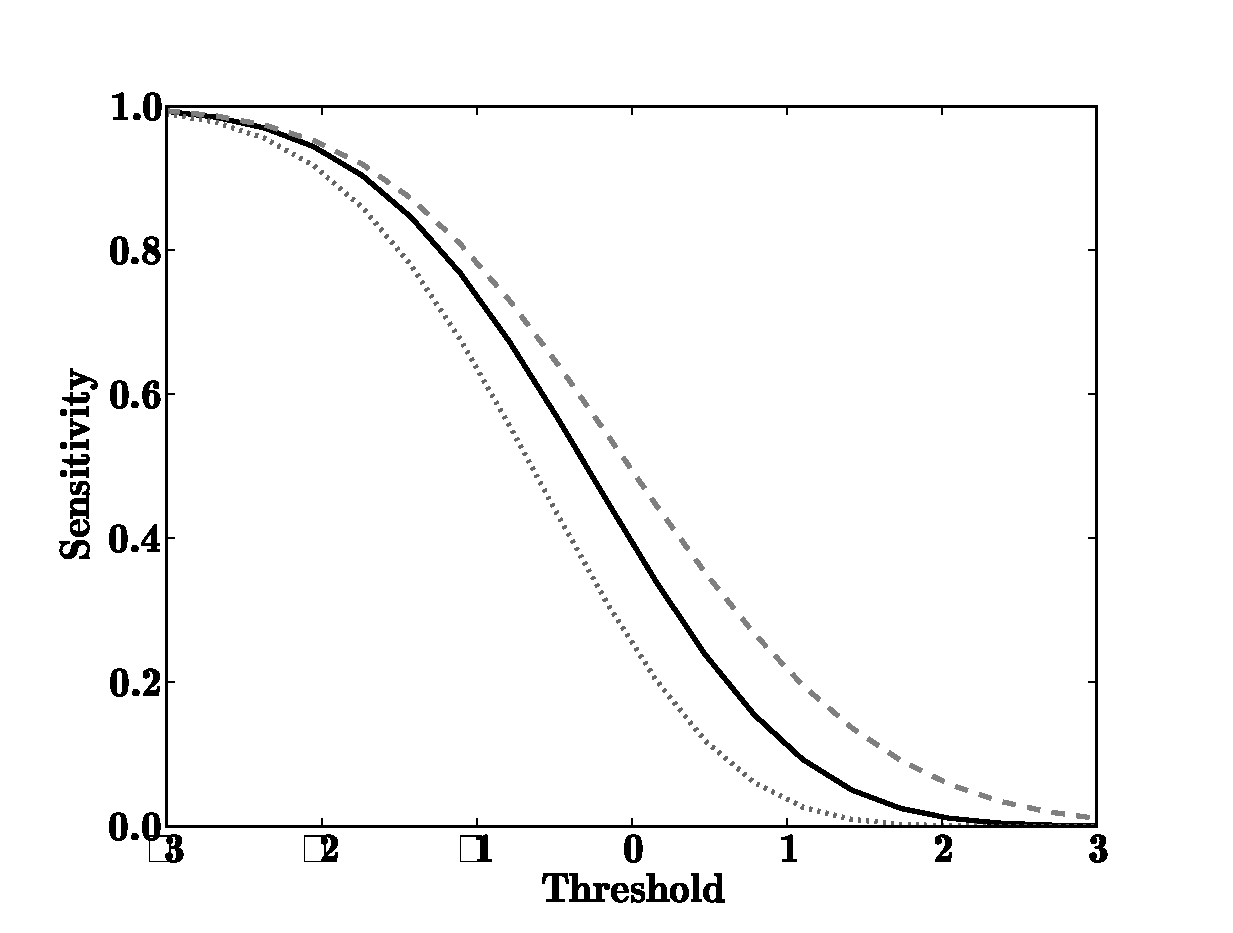
\includegraphics[width=.49\textwidth]{figs/sens_comparison_leafs}}
\subfigure[][]{\label{fig:1b}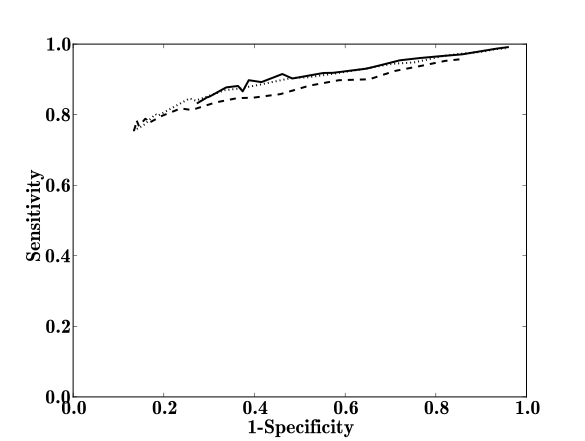
\includegraphics[width=.3\textwidth]{figs/amazon_pred_varying_mu}}
\subfigure[][]{\label{fig:clinical_roc}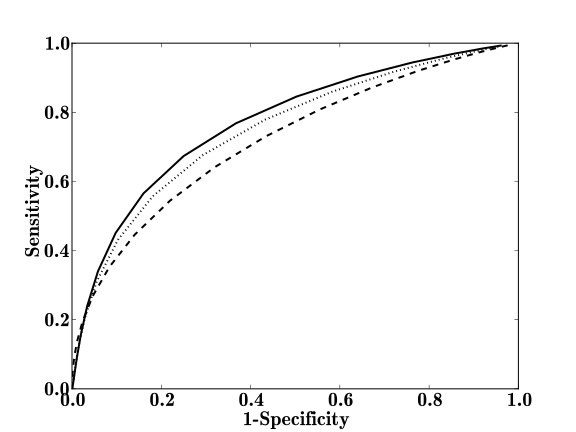
\includegraphics[width=0.3\textwidth]{figs/ROC_comparison_leafs}}
\caption{ROC curves for out-of-sample ICD-9 code prediction from patient free-text discharge records 
(\subref{fig:1a},\subref{fig:clinical_roc}). ROC curve for out-of-sample Amazon product category predictions from 
product free-text descriptions \subref{fig:1b}. Figures \subref{fig:1a} and \subref{fig:1b} are a function 
of the prior means of the regression parameters. Figure \subref{fig:clinical_roc} is a function of auxiliary variable threshold. In all figures, solid is 
HSLDA, dashed are independent regressors + sLDA (hierarchical 
constraints on labels ignored), and dotted is HSLDA fit by running LDA first then running 
tree-conditional regressions.}
\label{fig:main_results}
\end{center}
\end{figure}


The results in Figures~\ref{fig:1a} and \ref{fig:1b} suggest that in most cases
it is better to do full joint estimation of HSLDA.  An alternative
interpretation of the same results is that, if one is more sensitive to the
performance gains that result from exploiting the structure of the labels, then
one can, in an engineering sense, get nearly as much gain in label prediction
performance by first fitting LDA and then fitting a hierarchical probit
regression.  There are applied settings in which this could be advantageous.
